%!TEX root = main.tex

\subsection{数据集}

\begin{table*}
\footnotesize
\caption{平均关节误差(mm) on Human3.6M \cite{ionescu2014human} 给定2D位置}\label{tab:hm36m_rec}
\centering
% \renewcommand{\arraystretch}{0.3}
% \begin{tabularx}{l*{15}{c}}
\setlength{\tabcolsep}{1mm}{
\begin{tabular}{lcccccccc}
\toprule
 & Directions & Discussion & Eating & Greeting & Phoning & Photo & Posing & Purchases \\
\toprule
PMP  \cite{ramakrishna2012reconstructing}  &     127.6 &        134.8 &        127.6 &        144.7 &        129.7 &        138.4 &        137.0 &        146.2 \\
NRSFM \cite{dai2012simple}  &  137.2 &        140.7 &        129.8 &        118.0 &        134.3 &        120.0 &        156.5 &        161.7 \\
Convex \cite{zhou2015sparse} & 94.8 &         89.7 &         83.3 &         99.1 &         85.2 &        109.2 &         95.3 &         84.9 \\
Orth.  & 92.8 &         88.2 &         82.3 &         97.4 &         83.3 &        107.1 &         93.2 &         83.7         \\
Persp.  & 73.5 &         68.0 &         81.5 &         77.5 &         71.0 &         90.8 &         72.9 &         77.3         \\
\toprule
 & Sitting & SittingDown & Smoking & Waiting & WalkDog & Walking & WalkTogether & Average \\
 \toprule
PMP  \cite{ramakrishna2012reconstructing}  &  149.8 &        161.5 &        132.0 &        156.7 &        120.2 &        159.3 &        159.8 &        141.4 \\
NRSFM \cite{dai2012simple} &  180.6 &        177.2 &        127.2 &        137.2 &        136.8 &        104.7 &        113.6 &        136.9 \\
Convex \cite{zhou2015sparse} & 80.3 &         97.2 &         82.2 &         94.4 &         83.4 &         81.4 &         92.3 &         90.2 \\
Orth. & 79.0 &         96.8 &         80.9 &         92.4 &         81.6 &         81.5 &         91.3 &         88.7 \\
Persp.  & 68.3 &         91.4 &         66.8 &         75.0 &         67.0 &         60.1 &         71.5 &         74.2 \\
\toprule
\end{tabular}}
\end{table*}

% \begin{table}[ht]
%   \caption{\label{tab:sample}自动调节列宽的表格}
%   \begin{tabularx}{\linewidth}{c|XXXXXXXXXXXXXXX}
%       \hline
%       & Directions & Discussion & Eating & Greeting & Phoning & Photo & Posing & Purchases \\
%   \end{tabularx}
% \end{table}

\begin{table}
\caption{平均重建误差 (mm) on Human3.6M \cite{ionescu2014human} 给定关节位置.}\label{tab:nrsfm}
\centering
\renewcommand{\arraystretch}{1.5}
\begin{tabular}{l*{15}{c}}
\toprule
 & \cite{ramakrishna2012reconstructing} &  \cite{dai2012simple} & \cite{zhou2015sparse} & \cite{yasin2016dual} & Orth. & Persp. \\
\toprule
Protocol I & 90.9 & 82.9 & 51.3 & - & 51.1 & 50.5 \\
Protocol II & - & - & - & 70.5 & 55.1 & 54.6 \\
\toprule
\end{tabular}
\end{table}

对四个标准数据集进行了实证评估 -  Human3.6M \cite{ionescu2014human},Human Eva I \cite{sigal2010humaneva},KTH Football II \cite{kazemi2013multi}和MPII \cite{andriluka14cvpr}。 这些数据集涵盖了受控实验室和更现实的场景。 前三个数据集用于定量评估,最后一个用于定性评估。
\subsection{Evaluation metric} % (fold)
\label{sub:evaluation_metric}

给定3D关节位置$\hat\bfx_1,\cdots,\hat\bfx_n$ 与对应的真实位置$\bfx_1^*,\cdots,\bfx_n^*$ , \textbf{per joint error} 的定义是所有关节的欧式距离的均值:
\begin{align}\label{eq:pje}
e = \frac{1}{n}\sum_{i=1}^n\|\hat\bfx_i-\bfx_i^*\|_2.
\end{align}

请注意,上述指标取决于估计结构的绝对姿态,包括比例,平移和方向。 尺度和深度模糊是单眼重建所固有的,并且通常无法解决。 该尺度直接从基于预测的方法的训练对象中学习\cite{ionescu2014human,li2015,tekin2015}。 为了公平比较,我们的重建输出被缩放,使得平均肢长与所有训练对象的平均值相同。 作为Human3.6M和HumanEva数据集中的标准协议,比较骨架的根位置是对齐的,以使评估转换不变。 %请注意,不允许Procrustes与基础事实保持一致。

\textbf{reconstruction error} 为通过相似变换之后的3D关节误差, $\mathcal{T}$:
\begin{align*}
r = \min_{\mathcal{T}}\frac{1}{n}\sum_{i=1}^n\|\hat\bfx_i-\mathcal{T}(\bfx_i^*)\|_2,
\end{align*}
其中,通过Procrustes比对获得最佳参数。 三维重建误差广泛用于运动结构,以评估恢复结构的精度,无论尺度和刚性姿态如何。
\textbf{正确部件百分比(PCP)}定义为
\begin{align}\label{eq:pcp}
\mbox{PCP} = \frac{1}{n}\sum_{i=1}^n \mathbb{I}\left(\frac{\|\hat{\bfx}_i-\bfx_i\|+\|\hat{\bfy}_i-\bfy_i\|}{2\|\bfx_i-\bfy_i\|}\leq \tau\right),
\end{align}
其中$\bfx_i$和 $\bfy_i$是$i$ -th部分两端的坐标,$\hat\bfx_i$和$\hat\bfy_i$是相应的估计值。$\mathbb{I}$和$\tau$分别表示指标函数和阈值。 PCP指标衡量相对于给定阈值的正确定位部分的比例(在此工作中$\tau=0.5$)。

\subsection{Human3.6M}
\label{sec:h36m}

\begin{table*}
\footnotesize
\caption{Human3.6M上的每个关节误差(mm)的平均值 \cite{ionescu2014human}.标记$\dagger$表示使用序列信息。}
\centering
\renewcommand{\arraystretch}{0.5}
\renewcommand{\tabcolsep}{0.1 mm}
\begin{tabular}{l*{15}{c}}
\toprule
 & Directions & Discussion & Eating & Greeting & Phoning & Photo & Posing & Purchases \\
\toprule
LinKDE \cite{ionescu2014human} & 132.7 & 183.5 & 132.3 & 164.3 & 162.1 & 205.9 & 150.6 & 171.3 \\
Li et al. \cite{li2015} & - & 136.8 & 96.9 & 124.7 & - & 168.6 & - & - \\
Tekin et al. \cite{tekin2015}$^\dagger$ & 102.4 & 147.7 & 88.8 & 125.2 & 118.0 & 182.7 & 112.3 & 129.1 \\
Du et al. \cite{du2016marker}$^\dagger$  &        85.0 &       112.6 &        104.9 &        122.0 &        139.0 &        135.9 &        105.9 &        166.1 \\
Park et al. \cite{park20163d}  &         100.3 &        116.1 &        89.9 &        116.4 &        115.3 &        149.5 & 117.5 &        106.9 \\
Zhou et al. \cite{zhou2016deep}  &        91.8 &        102.4 &        96.6 &        98.7 &        113.3 &        125.2 &       90.0 &        93.8 \\
%Zhou et al. \cite{zhou2016sparseness} & {87.3} & {109.3} & {87.0} & {103.1} & {116.1} &  {143.3} & {106.8} & {99.7} \\
Generic+nonspecific$^\dagger$ & 82.8 &         88.2 &         93.3 &         93.0 &        111.7 &        115.9 &         85.4 &        131.4 \\
Generic+specific$^\dagger$ & 71.8 &         84.6 &         85.4 &         84.4 &        106.6 &        120.4 &         81.7 &        128.6 \\
Fine-tuned+nonspecific$^\dagger$ & 77.8 &         74.0 &         85.0 &         83.7 &         80.1 &         96.4 &         79.2 &         85.3 \\
Fine-tuned+specific$^\dagger$ & 69.2 &         75.2 &         75.8 &         73.6 &         75.4 &         99.6 &         76.1 &         73.6 \\
Fine-tuned+specific w/o smooth & 71.4 &         77.0 &         75.7 &         77.2 &         76.6 &        102.3 &         79.3 &         75.0 \\
\toprule
 & Sitting & SittingDown & Smoking & Waiting & WalkDog & Walking & WalkTogether & Average \\
\toprule
LinKDE \cite{ionescu2014human} & 151.5 & 243.0 & 162.1 & 170.6 & 177.1 & 96.6 & 127.8 & 162.1  \\
Li et al. \cite{li2015} & - & - & - & - & 132.1 & 69.9 & - & - \\
Tekin et al. \cite{tekin2015}$^\dagger$ & 138.8 & 224.9 & 118.4 & 138.7 & 126.2 & {55.0 }& {65.7 }& 124.9  \\
Du et al. \cite{du2016marker}$^\dagger$  &        117.4 &       226.9&        120.0 &        117.6 &        137.3 &        99.2 &        106.5 &        126.4 \\
Park et al. \cite{park20163d}  &         137.2 &        190.8 &        105.7 &        125.1 &       131.9 &        62.6 &        96.1 &        117.3 \\
Zhou et al. \cite{zhou2016deep}  &        132.1 &        158.9 &        106.9 &        94.4 &        126.0 &        79.0 &        98.9 &        107.2 \\
%Zhou et al. \cite{zhou2016sparseness} & {124.5} & {199.2} & {107.4} & {118.0} & {114.2} & 79.3 & 97.7 & {113.0} \\
Generic+nonspecific$^\dagger$ & 126.8 &        226.8 &         97.6 &         91.7 &         99.7 &         83.5 &         88.4 &        107.8 \\
Generic+specific$^\dagger$ & 114.9 &        225.1 &         93.3 &         99.0 &         95.6 &         65.0 &         74.9 &        102.2 \\
Fine-tuned+nonspecific$^\dagger$ & 79.1 &        118.4 &         75.3 &         80.3 &         75.3 &         67.8 &         81.8 &         82.7 \\
Fine-tuned+specific$^\dagger$ & 75.0 &        109.6 &         73.7 &         88.9 &         71.8 &         55.6 &         73.5 &         77.8 \\
Fine-tuned+specific w/o smooth &         76.0 &        112.2 &         74.2 &         91.3 &         73.1 &         57.8 &         74.1 &         79.6 \\
\toprule
\end{tabular}
\label{tab:h36m}
\end{table*}

\begin{table*}
  \footnotesize
\caption{Human3.6M上的平均重建误差(mm) \cite{ionescu2014human}.}
\centering
\renewcommand{\arraystretch}{0.5}
\renewcommand{\tabcolsep}{0.1 mm}
\begin{tabular}{l*{15}{c}}
\toprule
 & Directions & Discussion & Eating & Greeting & Phoning & Photo & Posing & Purchases \\
\toprule
SMPLify \cite{bogo2016keep} & 62.0 & 60.2 & 67.8 & 76.5 & 92.1 & 77.0 & 73.0 & 75.3 \\
Generic+nonspecific & 52.0 &         54.0 &         59.1 &         61.7 &         74.2 &         70.7 &         51.5 &         60.3 \\
%Generic+specific & 48.2 &         54.3 &         52.5 &         57.8 &         69.6 &         73.9 &         52.9 &         62.2 \\
Fine-tuned+nonspecific & 46.7 &         47.7 &         54.9 &         54.1 &         56.3 &         65.4 &         46.9 &         49.1 \\
%Fine-tuned+specific &  44.2 &         50.5 &         52.0 &         51.3 &         54.6 &         67.6 &         48.9 &         46.4 \\
\toprule
 & Sitting & SittingDown & Smoking & Waiting & WalkDog & Walking & WalkTogether & Average \\
\toprule
SMPLify \cite{bogo2016keep} & 100.3 & 137.3 & 83.4 & 77.3 & 79.7 & 86.8 & 81.7 & 82.3 \\
Generic+nonspecific & 83.9 &        119.9 &         66.9 &         54.8 &         64.5 &         55.6 &         59.1 &         65.9 \\
%Generic+specific & 75.2 &        117.7 &         65.2 &         59.4 &         62.7 &         46.7 &         50.7 &         63.3 \\
Fine-tuned+nonspecific & 60.1 &         81.5 &         53.2 &         49.7 &         54.2 &         47.1 &         53.7 &         54.7 \\
%Fine-tuned+specific &  57.9 &         74.6 &         53.6 &         54.6 &         52.2 &         41.0 &         47.7 &         53.2 \\
\toprule
\end{tabular}
\label{tab:h36m1}
\end{table*}

\begin{table*}
\footnotesize
\caption{Human3.6M在线测试集上的平均关节误差(``H36M\_NOS10'') \cite{ionescu2014human}.}
\centering
\renewcommand{\arraystretch}{0.5}
\renewcommand{\tabcolsep}{0.1 mm}
\begin{tabular}{l*{15}{c}}
\toprule
 & Directions & Discussion &	Eating &	Greeting &	Phoning &	Posing &	Purchases &	Sitting \\
\toprule
Ionescu et al. \cite{ionescu2014human} & 117&	108&	91&	129&	104&	130&	134&	135 \\
Li et al. \cite{li2015} & - & 92& 76& 98& 92& 107& 141& 136 \\
Grinciunaite et al. \cite{grinciunaite2016human} & 91&	89&	94&	102&	105&	99&	112&	151 \\
Proposed & 78   &    74    &   86 &	80   &    89	& 93	& 76    &   95	\\
\toprule
 & SittingDown &	Smoking	& Photo &	Waiting &	Walking &	WalkDog &	WalkTogether &    Mean \\
\toprule
Ionescu et al. \cite{ionescu2014human} & 200&	117&	195&	132&	115&	162&	156&	133  \\
Li et al. \cite{li2015} & 265 & 97& 171& 105& 99& 139& 110& 122 \\
Grinciunaite et al. \cite{grinciunaite2016human} & 239&	109&	151&	106&	101&	141&	106&	119 \\
Proposed & 114  &   83	& 101 &	91 &	64	& 87	& 71 &           86\\
\toprule
\end{tabular}
\label{tab:h36m_test}
\end{table*}

Human3.6M \cite{ionescu2014human}是最近用于3D人体感知的大型数据集。 它包括从MoCap系统获取的数百万个3D人体姿势以及来自校准相机的相应图像。
此设置提供同步视频和2D-3D姿势数据以供评估。 它包括11个主题,执行15个动作,如吃饭,坐着和走路。 使用与先前工作相同的数据分区协议\cite{li2015,tekin2015}:来自五个类别(S1,S5,S6,S7,S8)的数据用于训练,并且来自两个类别的数据(S9,S11) )用于测试。 原始帧速率为50 fps,并下采样为10 fps。

% \subsubsection{具有已知2D姿势的3D姿势重建}
 
% 首先,给出了具有已知2D姿势的所提出方法的3D可重构性的评估。 通过序列的2D对应的3D重建的通用方法是NRSFM。 将所提出的方法与人类3.6M上的NRSFM \cite{dai2012simple}中的最新技术进行了比较。 最近的单视图姿势重建方法,投影匹配追踪(PMP)\cite{ramakrishna2012reconstructing},以及我们的管道中使用的初始化方法\cite{zhou2015sparse}也包括在比较中。

% All sequences of S9 and S11 in Human3.6M were used for evaluation. A single pose dictionary from all the training pose data, irrespective of the action type, was used, i.e., a non-action specific dictionary. Dai et al.'s approach \cite{dai2012simple} requires a predefined rank $K$.  Various values of $K$ were considered with the best result for each sequence reported.

% The per joint errors for each action are presented in \refTab{tab:hm36m_rec}, while the reconstruction errors are summarized in \refTab{tab:nrsfm}. In \refTab{tab:nrsfm}, Protocol I means the protocol introduced above in this paper, and Protocol II is the one proposed in \cite{yasin2016dual} where only S11 and 14 joints are used in evaluation. The proposed approach  with a perspective model (``Persp.") outperforms its orthographic counterpart (``Orth.") by a large margin in terms of per joint error.
% This performance difference is mostly due to the inaccuracy of rigid pose estimation with the orthographic model, which greatly increases the per joint error as Procrustes alignment is not allowed in the evaluation. Moreover, the orthographic model may suffer from a reflection ambiguity.  
% In terms of reconstruction error which ignores rigid pose, the difference between the perspective and orthographic models is much smaller.

% ``Orth." performs slightly better than the initialization approach \cite{zhou2015sparse}. Note, given the 2D joints, 
% %if the 2D joints are given, 
% ``Orth." reduces to the initialization approach 
% %\cite{zhou2015sparse} 
% combined with temporal smoothness constraints.

% The proposed approach also outperforms the NRSFM baseline  \cite{dai2012simple}. The main reason is that the videos are captured by stationary cameras. Although the subject is occasionally rotating, the ``baseline" between frames is generally small, and neighboring views provide insufficient geometric constraints for 3D reconstruction. In other words, NRSFM is very difficult to solve in the case of slow camera motion. This observation is consistent with prior findings in the NRSFM literature, e.g., \cite{akhter2011trajectory}. In this case, the structure prior (even a non-action specific one) learned from existing MoCap data is critical for reconstruction.

% \subsubsection{3D pose reconstruction with unknown 2D pose}

% Next, results on the Human3.6M dataset are reported when 2D poses are predicted from images using the CNN described in \refSec{sec:cnn}. The proposed approach is compared to several recent baselines including both discriminative approaches (e.g., \cite{ionescu2014human,li2015,tekin2015}) and two-stage reconstruction approaches (e.g., \cite{bogo2016keep}). For the proposed approach, four combinations of training data sources were considered -- the generic hourglass model trained on MPII (``generic'') or the fine-tuned model trained on Human3.6M (``fine-tuned'') combined with the nonspecific dictionary learned with all 3D pose data (``nonspecific'') or the dictionary learned with action specific pose data (``specific'').

% The mean per joint errors are summarized in \refTab{tab:h36m}. The table shows that the proposed approach outperforms the baselines on most of the actions, yielding a much lower average error compared to the baselines. The ``walk" and ``walk together" sequences involve very predictable and repetitive motions. This might favor the direct regression approach \cite{tekin2015}. The reconstruction errors are provided in \refTab{tab:h36m1}. The proposed approach with a generic 2D pose detector outperforms SMPLify \cite{bogo2016keep}, which is the state-of-the-art two-stage approach that reconstructs 3D poses by fitting a parametric body shape model to 2D joints detected by a CNN-based 2D pose detector.

% Comparing the results using different sources of training data, a remarkable improvement was achieved by using the fine-tuned 2D pose detector and the action specific 3D pose dictionaries. Nevertheless, the proposed approach with the generic detector and non-action specific dictionary still attained very competitive performance compared to the state-of-the-art. Note that the proposed approach can also be applied to single frames without temporal smoothness, with corresponding results presented in the last row of \refTab{tab:h36m}. 

% \subsubsection{Human3.6M online test set}
% \refTab{tab:h36m_test} presents results on the Human3.6M online test set ``H36M\_NOS10''.  The test set includes 360 sequences from three subjects with hidden ground truth. As the standard protocol, all compared approaches used action specific training. 
% We used the fine-tuned hourglass model and action specific dictionaries. The results show that the proposed approach achieves significant improvements for all actions compared to the previous approaches.

% \subsubsection{Ablative analysis}

% \refTab{tab:steps} shows the impact of each component in our approach. For our approach, the 2D pose estimates were obtained from the expectations of their posterior distributions given in \refEq{eq:der2}. Note that the 2D errors are with respect to the normalized bounding box size $256\times256$. Two cases of 2D input were considered: heat maps from the generic detector (less accurate), and the fine-tuned detector (more accurate).  In this evaluation, action specific pose dictionaries and the Stacked Hourglass for joint heat map prediction were used.%  in our evaluation.

% \refTab{tab:steps} suggests that, for the same model, both the 3D and 2D errors increase significantly if EM is not applied.  This indicates the importance of marginalizing the 2D uncertainty. Removing the smoothness constraint also increases the error, while the difference is more apparent when the 2D input is more noisy (from the ``generic" detector). The perspective model always outperforms the orthographic model %, but the 
% with the gap in terms of per joint error being much larger than that of reconstruction error.  This indicates that the performance gain using a perspective camera model is mainly due to the more accurate rigid pose estimation. Finally, with the same orthographic model, the proposed approach clearly improves the initial solution \cite{zhou2015sparse} by taking advantage of EM and smoothness.

% An alternative to the proposed EM algorithm is the maximum a posteriori (MAP) estimation which minimizes $-\ln\pr(\bfI,\bfW|\theta)+\mathcal{R}(\theta)$ over $\theta$ and $\bfW$. We implemented the block coordinate descent to solve the MAP estimation. With the fine-tuned detector, the mean per joint error of MAP is 79.3 mm, which is worse than that of EM (77.8 mm).


\begin{table}
  \footnotesize
\caption{不同的方法的估计误差。 “PJ”,“Rec”和“2D”分别对应于每个关节误差(mm),重建误差(mm)和2D误差(像素)。}
\centering
\renewcommand{\arraystretch}{0.5}
\renewcommand{\tabcolsep}{0.1 mm}
\begin{tabular}{l*{15}{c}}
\toprule
& \multicolumn{3}{c}{Generic} & \multicolumn{3}{c}{Fine-tuned} \\
 & PJ & Rec  & 2D & PJ & Rec & 2D \\
\toprule
Perspective & 102.2 & 63.3 & 10.1 & 77.8 & 53.2 & 6.0 \\
w/o smooth & 106.0 & 65.0 & 10.2 & 79.6 & 54.1 & 6.0 \\
w/o smooth/EM & 108.1 & 67.2 & 11.3 & 81.4 & 55.3 & 6.5 \\
\hline
Orthographic & 118.4 & 64.4 & 10.1 & 92.5 & 55.6 & 6.0 \\
w/o smooth & 122.2 & 65.4 & 10.2 & 93.8 & 55.3 & 6.0 \\
w/o smooth/EM  \cite{zhou2015sparse} & 127.3 & 67.2 & 11.3 & 100.5 & 58.2 & 6.5 \\
\toprule
\end{tabular}
\label{tab:steps}
\end{table}

\subsubsection{对参数的敏感性}

\begin{figure}
  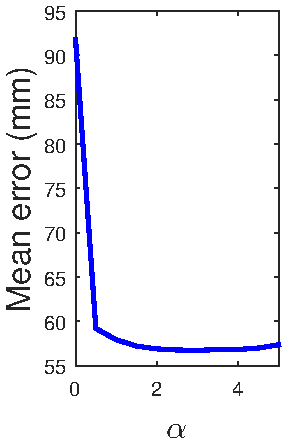
\includegraphics[width=0.32\linewidth]{figures/alpha.pdf} \hfill
  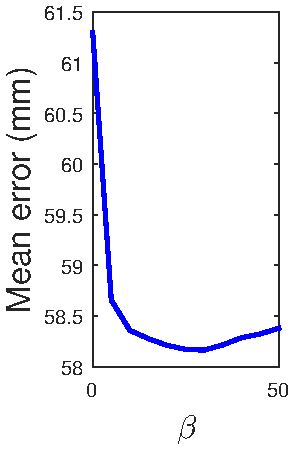
\includegraphics[width=0.32\linewidth]{figures/beta.pdf} \hfill
  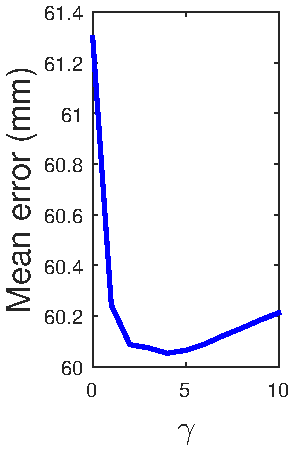
\includegraphics[width=0.32\linewidth]{figures/gamma.pdf}
  \caption{对模型参数的敏感性。 分别显示平均重建误差与模型参数$\alpha$,$\beta$或$\gamma$的关系。}\label{fig:par}
\end{figure}

\begin{figure*}
  \centering
  \begin{minipage}{0.49\textwidth}
  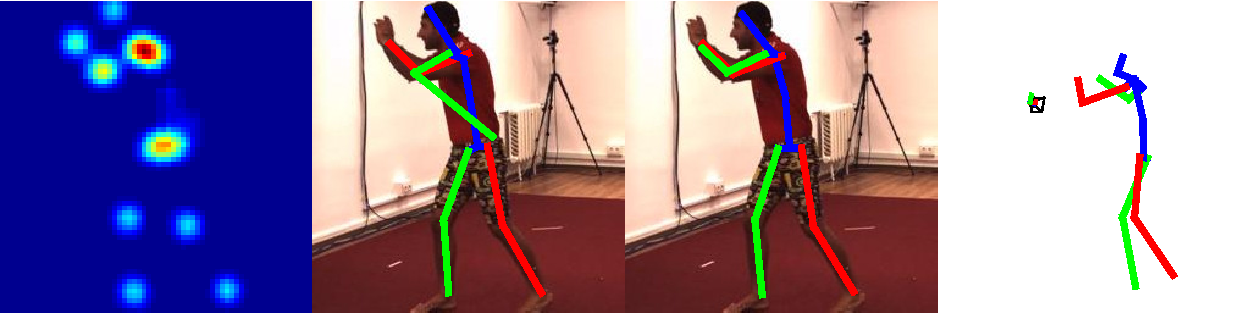
\includegraphics[width=\linewidth]{figures/examples/h36m/S9-1.pdf}\vspace{0.3em}
  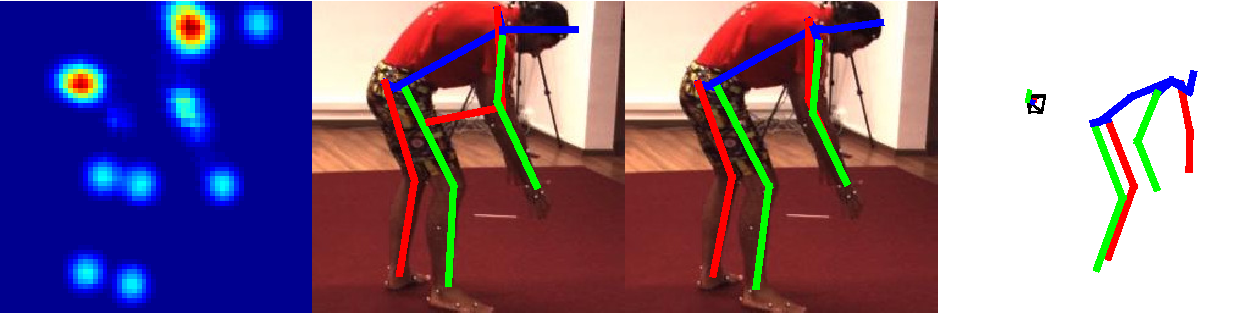
\includegraphics[width=\linewidth]{figures/examples/h36m/S9-2.pdf}\vspace{0.3em}
  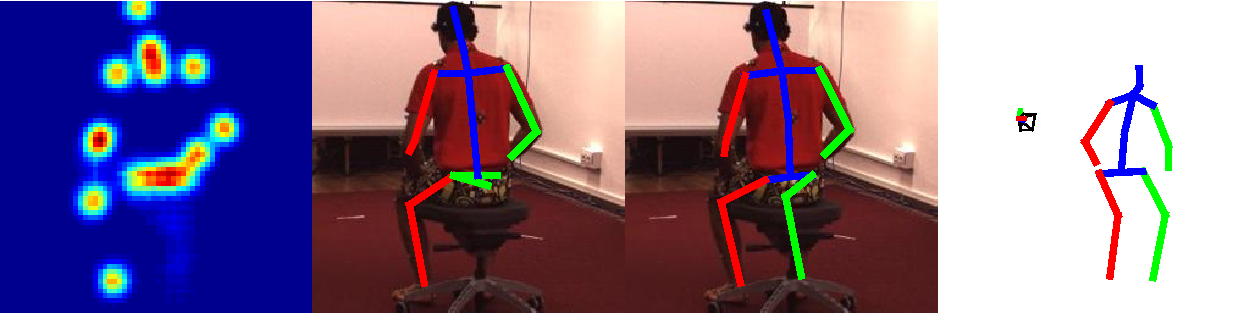
\includegraphics[width=\linewidth]{figures/examples/h36m/S9-3.pdf}\vspace{0.3em}
  % 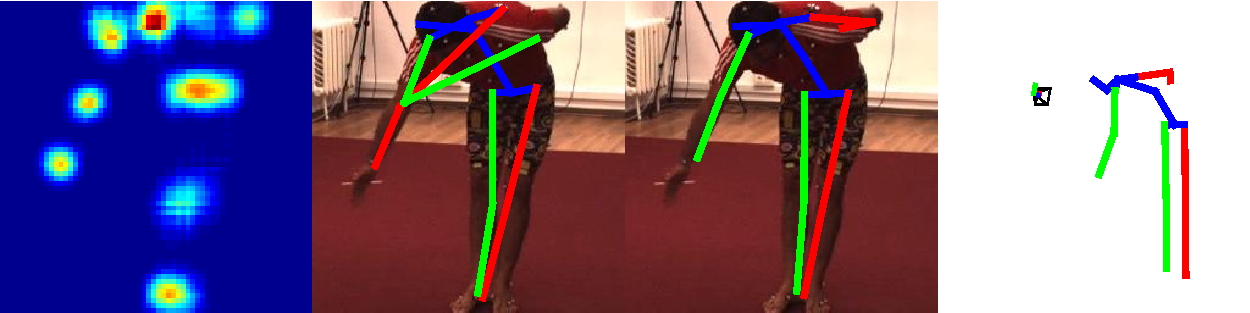
\includegraphics[width=\linewidth]{figures/examples/h36m/S9-4.pdf}\vspace{0.3em}
  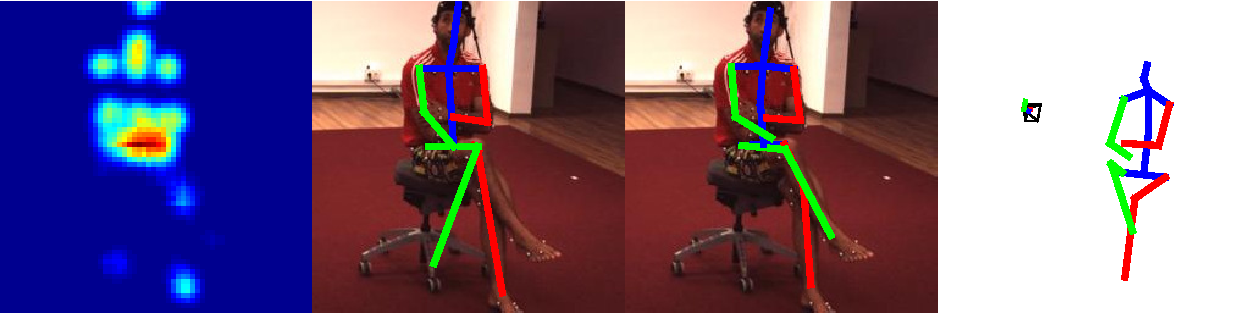
\includegraphics[width=\linewidth]{figures/examples/h36m/S9-5.pdf}\vspace{0.3em}
  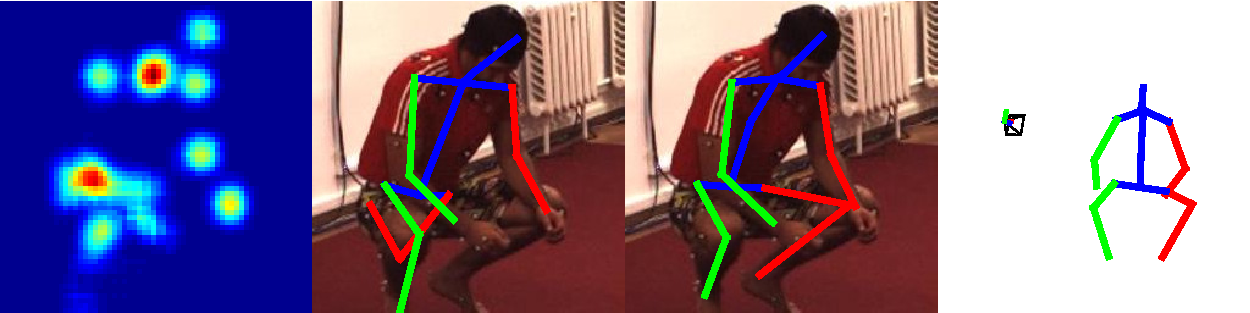
\includegraphics[width=\linewidth]{figures/examples/h36m/S9-6.pdf}\vspace{0.3em}
  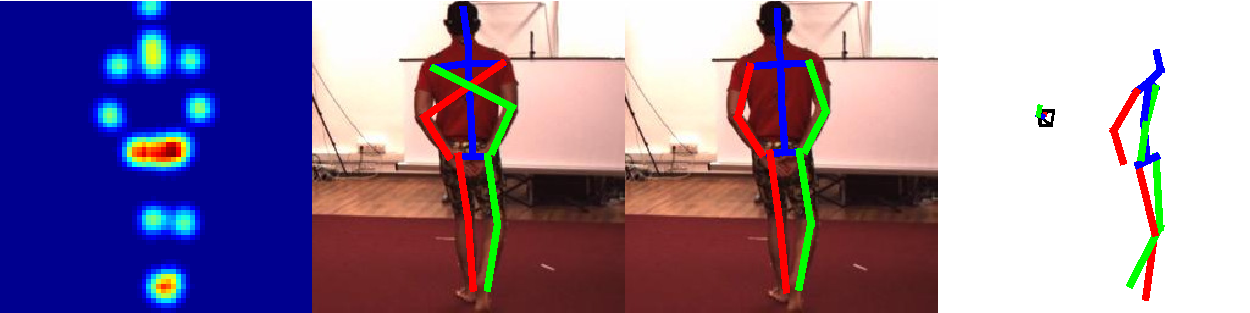
\includegraphics[width=\linewidth]{figures/examples/h36m/S9-7.pdf}\vspace{0.3em}
  \end{minipage}
  \begin{minipage}{0.49\textwidth}
  % 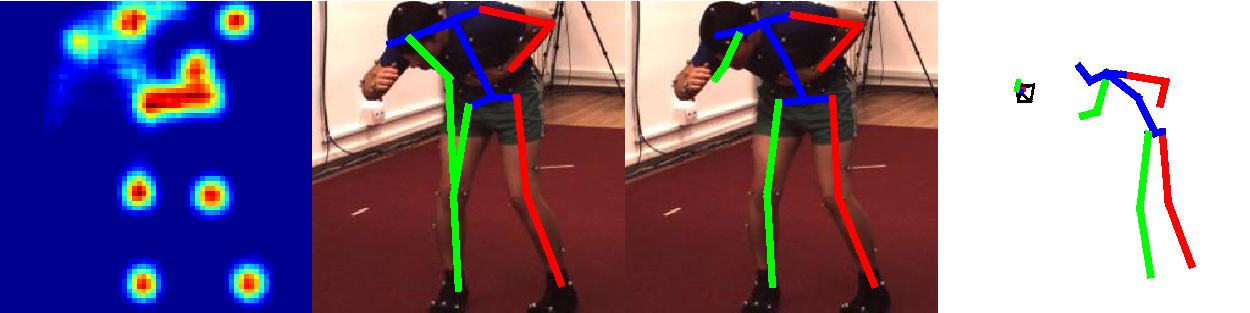
\includegraphics[width=\linewidth]{figures/examples/h36m/S11-1.pdf}\vspace{0.3em}
  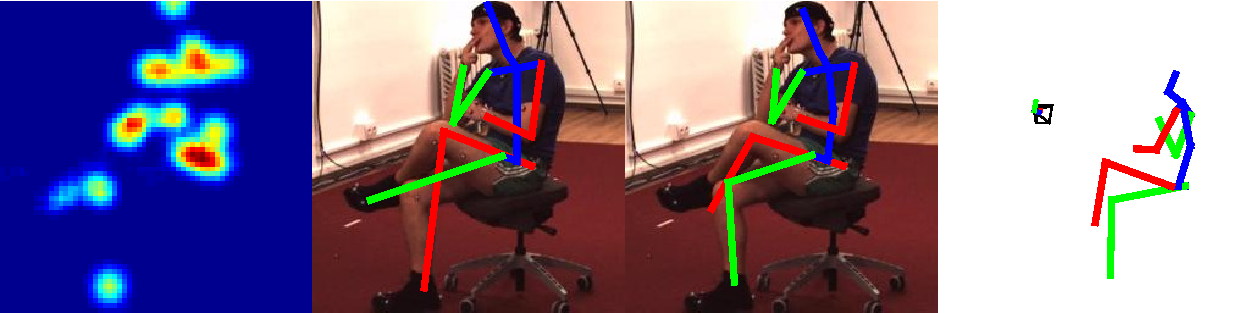
\includegraphics[width=\linewidth]{figures/examples/h36m/S11-2.pdf}\vspace{0.3em}
  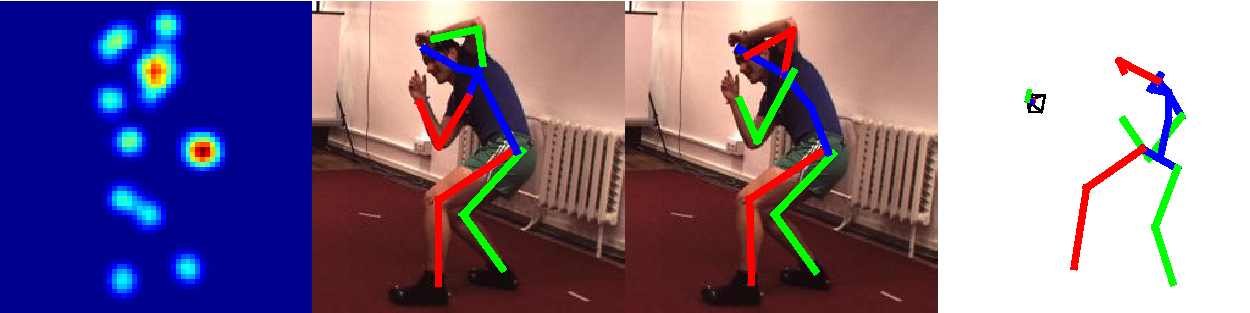
\includegraphics[width=\linewidth]{figures/examples/h36m/S11-3.pdf}\vspace{0.3em}
  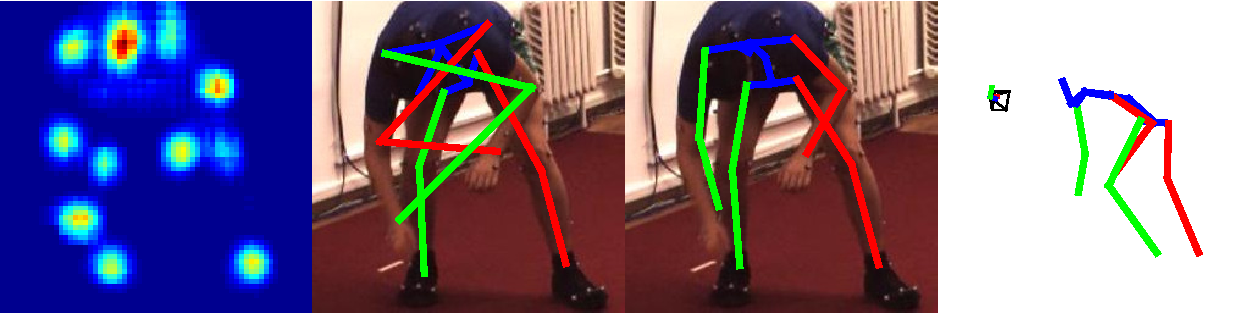
\includegraphics[width=\linewidth]{figures/examples/h36m/S11-4.pdf}\vspace{0.3em}
  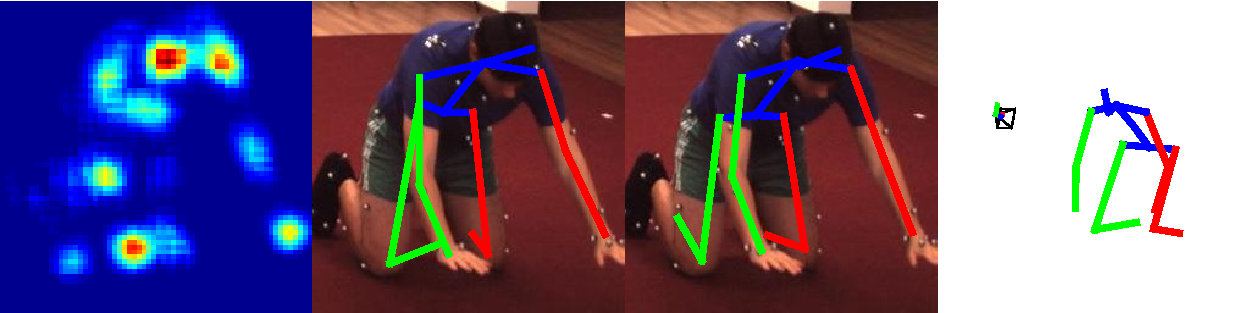
\includegraphics[width=\linewidth]{figures/examples/h36m/S11-5.pdf}\vspace{0.3em}
  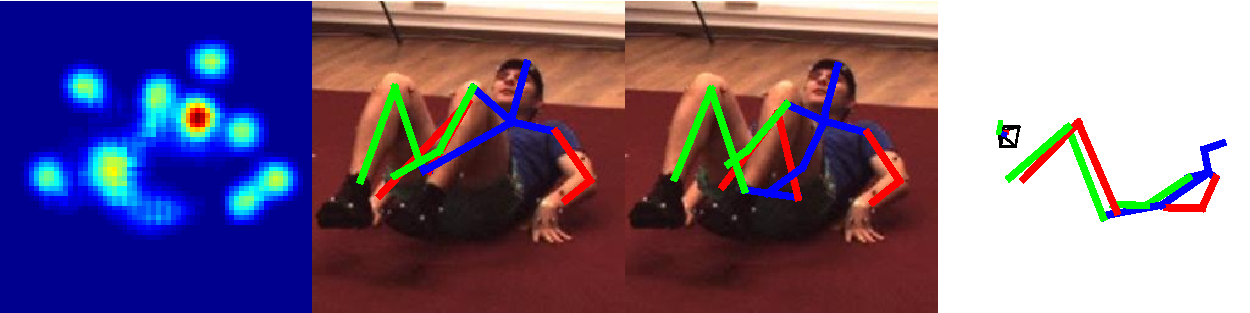
\includegraphics[width=\linewidth]{figures/examples/h36m/S11-6.pdf}\vspace{0.3em}
  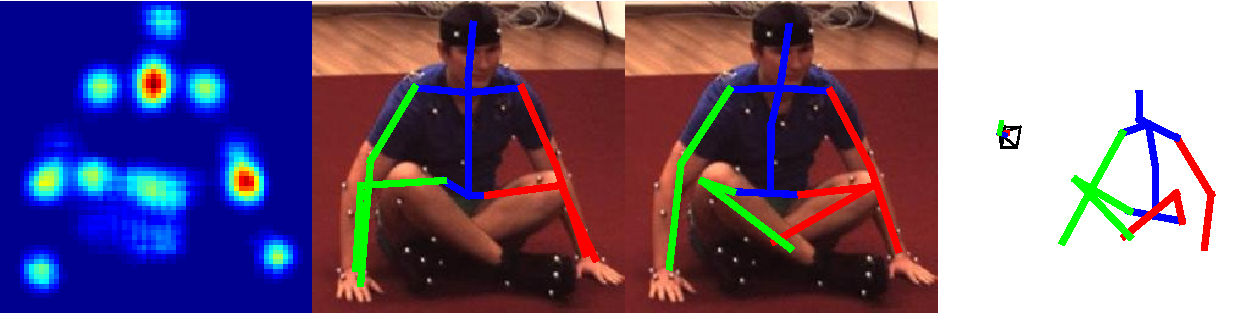
\includegraphics[width=\linewidth]{figures/examples/h36m/S11-7.pdf}\vspace{0.3em}
  \end{minipage}
  \caption{Human3.6M \cite{ionescu2014human}的比较框架结果示例。 每行包括两个示例。 从左到右的图像对应于热图(所有关节同时显示),通过根据热图分别贪婪地定位每个关节,通过所提出的EM算法估计的2D姿势以及估计的3D来找到2D姿势。 姿势在一种新颖的视角中可视化。 还显示了原始视点。 请注意,在考虑姿势和时间平滑度先验后,2D热图中的误差会得到纠正。 }\label{fig:h36m}
\end{figure*}

\begin{figure*}
  \centering
  % Requires \usepackage{graphicx}
  \begin{minipage}{0.48\textwidth}
  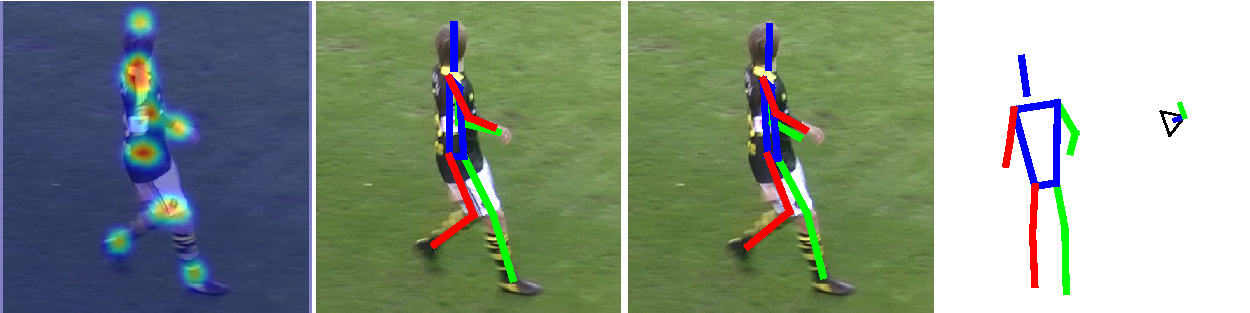
\includegraphics[width=0.95\linewidth]{figures/examples/kth/Seq1_C1-001.pdf}
  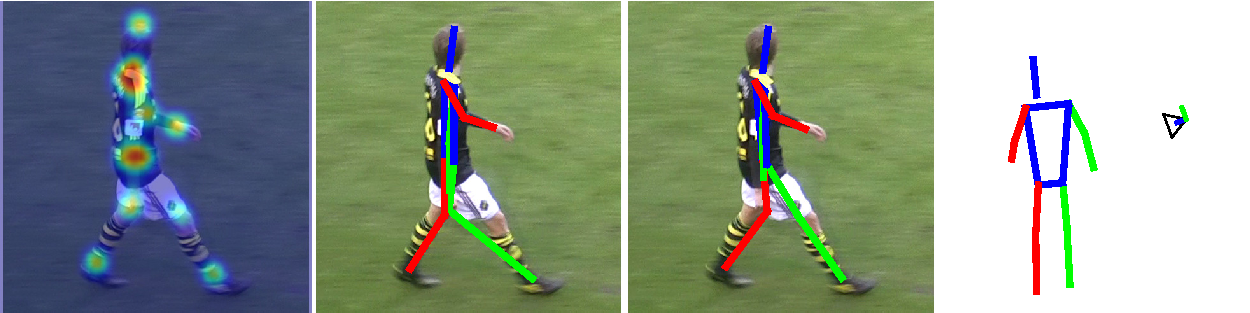
\includegraphics[width=0.95\linewidth]{figures/examples/kth/Seq1_C1-021.pdf}
  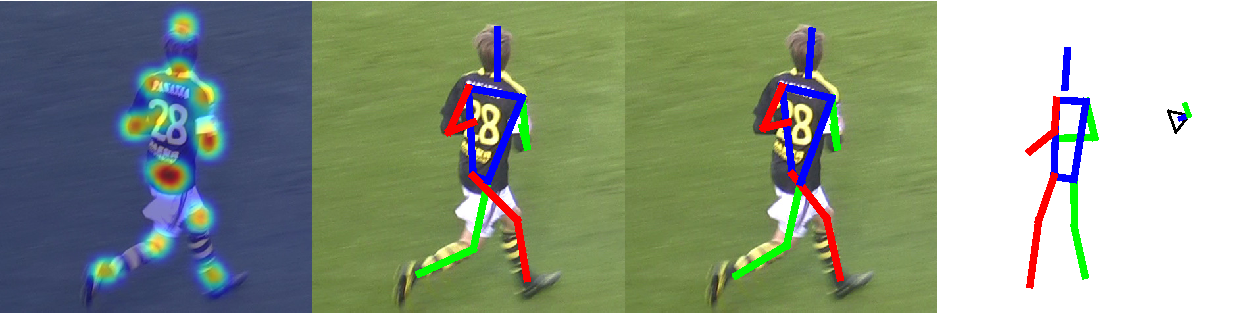
\includegraphics[width=0.95\linewidth]{figures/examples/kth/Seq1_C1-108.pdf}
  \end{minipage}
  \hfill
  \begin{minipage}{0.48\textwidth}
  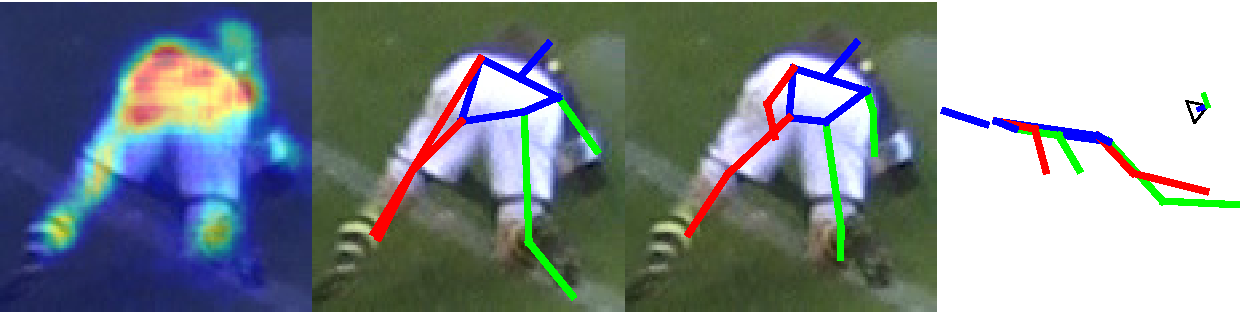
\includegraphics[width=0.95\linewidth]{figures/examples/kth/Seq2_C1-007.pdf}
  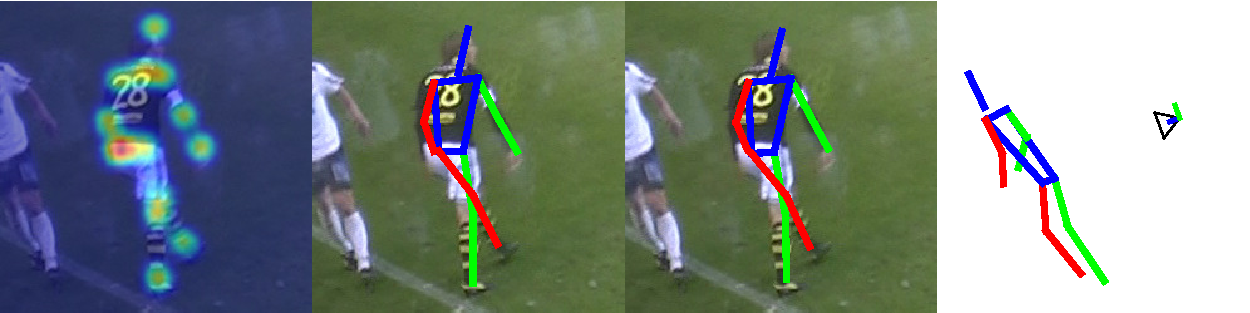
\includegraphics[width=0.95\linewidth]{figures/examples/kth/Seq2_C1-047.pdf}
  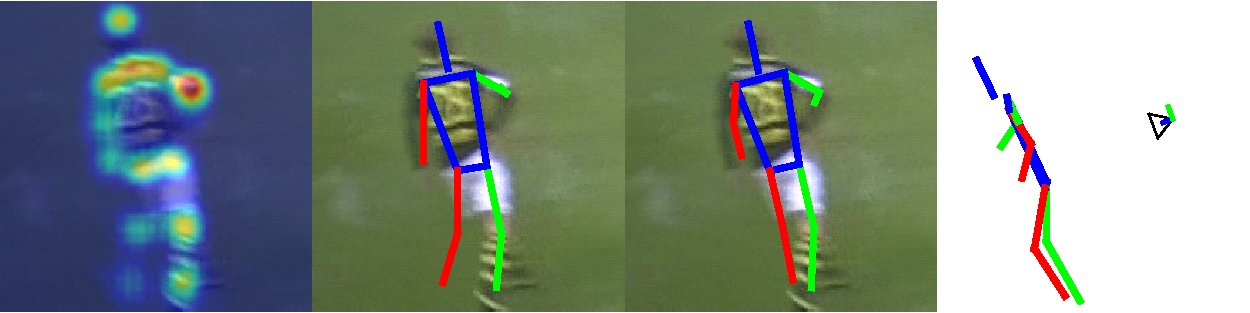
\includegraphics[width=0.95\linewidth]{figures/examples/kth/Seq2_C1-075.pdf}
  \end{minipage}
  \caption{ KTH Football II \cite{burenius20133d}的比较框架结果示例。 在每个示例中从左到右的图像对应于热图(所有关节同时显示),通过根据热图响应贪婪地定位每个关节而找到的2D姿势,通过所提出的EM算法估计的2D姿势, 并且在新颖的视图中可视化估计的3D姿势。 还显示了原始视点。}\label{fig:kth}
\end{figure*}

\begin{table*}
\caption{HumanEva I上的平均重建误差(mm)\cite{sigal2010humaneva}.}
\centering
\renewcommand{\arraystretch}{0.5}
\renewcommand{\tabcolsep}{0.1 mm}
\begin{tabular}{l*{3}{c}*{4}{c}}
\toprule
& \multicolumn{3}{c}{Walking} & \multicolumn{3}{c}{Jogging} & Average \\
& S1 & S2 & S3 & S1 & S2 & S3 \\
\toprule
Radwan et al. \cite{radwan2013monocular} & 75.1 & 99.8 & 93.8 & 79.2 & 89.8 & 99.4 & 89.5 \\
Wang et al. \cite{wang2014robust} & 71.9 & 75.7 & 85.3 & 62.6 & 77.7 & 54.4 & 71.3 \\
Simo-Serra et al. \cite{simo2013joint} & 65.1 & 48.6 & 73.5 & 74.2 & 46.6 & 32.2 & 56.7\\
Bo et al. \cite{bo2010twin} & 46.4 & {30.3} & 64.9 & 64.5 & 48.0 & 38.2 & 48.7 \\
Kostrikov et al. \cite{kostrikov2014depth} & 44.0 & 30.9 & 41.7 & 57.2 & 35.0 & 33.3 & 40.3 \\
Yasin et al. \cite{yasin2016dual} & 35.8 & 32.4 & {41.6} & {46.6} & 41.4 & 35.4 & 38.9 \\
Proposed & {34.3} & 31.6 & 49.3 & 48.6 & {34.0} & {30.0} & {37.9}\\
\toprule
\end{tabular}
\label{tab:humaneva}
\end{table*}

\refFig{fig:par}显示平均重建误差作为\refEq{eq:prior}中每个参数的函数,同时修复其他参数,在测试序列的子集上进行评估(来自S9的前五个动作)。 第一条曲线显示,当$\alpha$变为非零时,错误最初会迅速减少。 这表明稀疏性约束的重要性。 在初始快速减少之后,错误变化非常平滑,这表明当其值在适当范围内时,解决方案对$\alpha$不是非常敏感。 类似的观察结果是光滑度项的权重,$\beta$ 和$\gamma$。
实际上,在本文提出的所有其他实验中,模型参数是固定的而没有特定的调整(在标准化的2D坐标系中$\alpha=0.5$, $\beta=20$和$\gamma=2$)。

\subsubsection{定性说明}

\refFig{fig:h36m}在几个示例帧上可视化结果。 虽然热图可能由于遮挡,左右模糊以及来自检测器的其他不确定性来源而是错误的,但是所提出的EM算法可以通过利用姿势先验,积分时间平滑性和对不确定性建模来有效地校正误差。

\subsection{HumanEva I}


在本节中,将介绍HumanEva I \cite{sigal2010humaneva}的评估结果。其他地方描述的评估协议\cite{simo2013joint}被采用。来自所有受试者的摄像机C1的步行和慢跑序列用于评估。在Human3.6M上训练的2D关节探测器分别用每个动作的训练序列进行微调。针对每个主题分别学习具体行动的姿势词典。通过所提出的方法重建的每个3D姿势被缩放以具有与训练数据相同的平均肢长。
评估序列的平均重建误差记录在 \refTab{tab:humaneva}中。比较基线的结果取自先前的工作\cite{yasin2016dual}。由于训练和测试数据之间的重叠较大,姿势的可变性较小,
对于所有方法,与Human3.6M相比,通常在该数据集上获得更高的准确度。虽然没有一种方法在所有序列中占主导地位,但我们的整体准确度最高。

\subsection{KTH Football II}

KTH Multiview Football II \cite{kazemi2013multi}包含职业足球运动员比赛的图像。
它包括具有3D基础事实的图像序列,用于从三个校准视图捕获的14个注释关节。
使用手动2D注释的多视图重建生成3D地面实况。
我们的评估是使用标准协议\cite{tekin2015}进行的,其中来自“相机1”的“播放器2”的序列用于测试。在MPII上训练的通用沙漏模型被用作2D检测器而没有罚款 -tuning,同时使用与该数据集中提供的训练图像相关联的3D姿势来学习姿势字典。
通过所提出的方法重建的每个3D姿势被缩放以具有与训练姿势相同的平均肢长,然后通过根据根位置的平移与地面实况对齐。
为了与基线进行比较,报告的结果基于用于测量3D中的部件定位的正确姿势(PCP)的百分比。
\refTab{tab:kth}提供了PCP结果的摘要。 它表明,所提出的方法实现了比现有技术更高的准确性。 选定帧的结果在\refFig{fig:kth}中可视化。

\begin{table}
\caption{Mean PCP scores on KTH Football II \cite{burenius20133d}.}
\centering
\renewcommand{\arraystretch}{0.5}
\renewcommand{\tabcolsep}{0.1 mm}
\begin{tabular}{l*{3}{c}*{1}{c}}
\toprule
& \multicolumn{3}{c}{Sequence 1} & \multicolumn{1}{c}{Sequence 2} \\
& \cite{burenius20133d} & \cite{tekin2015} & Proposed & Proposed \\
\toprule
Upper Arms & 14 & 74 & {89} & 61\\
Lower Arms & 06 & 49 & {78} & 49\\
Upper Legs & 63 & 98 & {99} & 77\\
Lower Legs & 41 & 77 & {85} & 56\\
\toprule
\end{tabular}

\label{tab:kth}
\end{table}

\subsection{MPII}

\begin{figure*}
  \centering
  % Requires \usepackage{graphicx}
  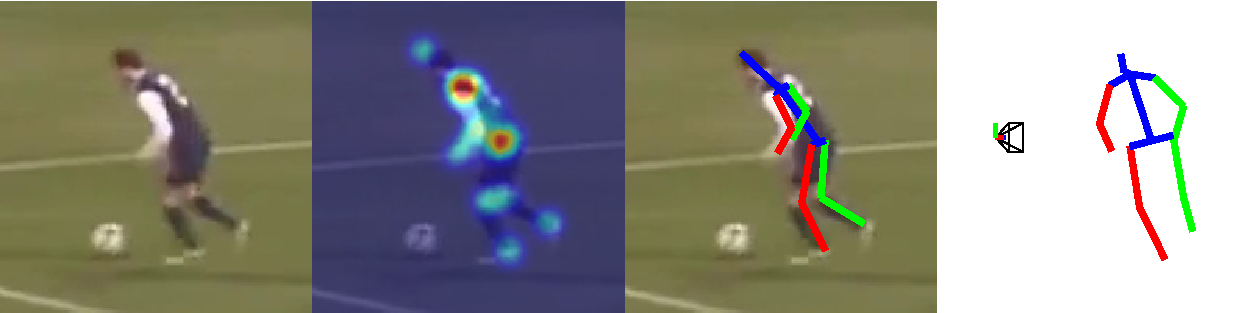
\includegraphics[width=0.48\linewidth]{figures/examples/mpii/mpii-001.pdf}
  %\includegraphics[width=0.48\linewidth]{figures/examples/mpii/mpii-002.pdf}
  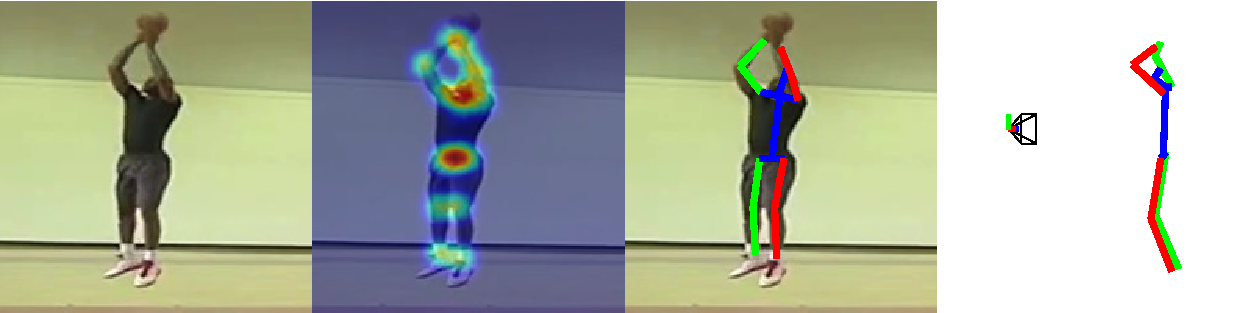
\includegraphics[width=0.48\linewidth]{figures/examples/mpii/mpii-004.pdf}
  % \includegraphics[width=0.48\linewidth]{figures/examples/mpii/mpii-006.pdf}
  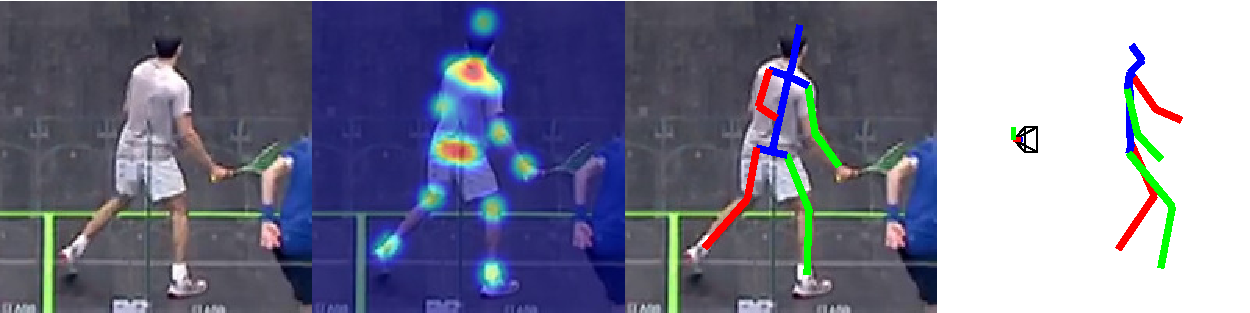
\includegraphics[width=0.48\linewidth]{figures/examples/mpii/mpii-010.pdf}
  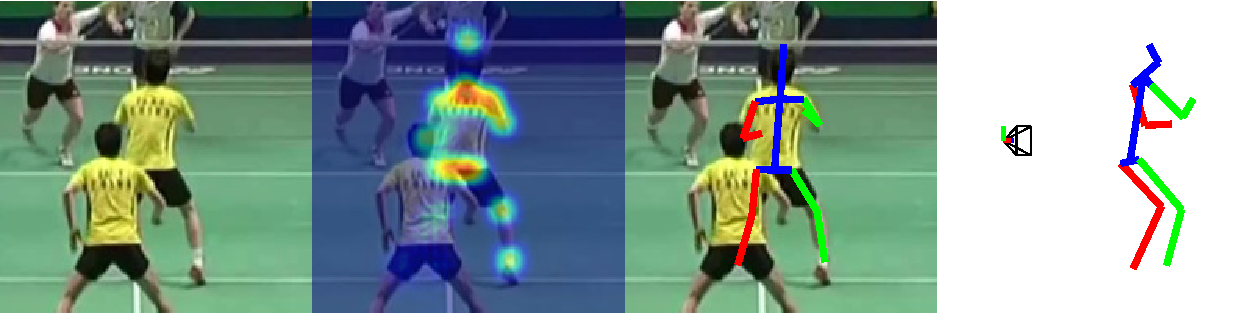
\includegraphics[width=0.48\linewidth]{figures/examples/mpii/mpii-014.pdf}
  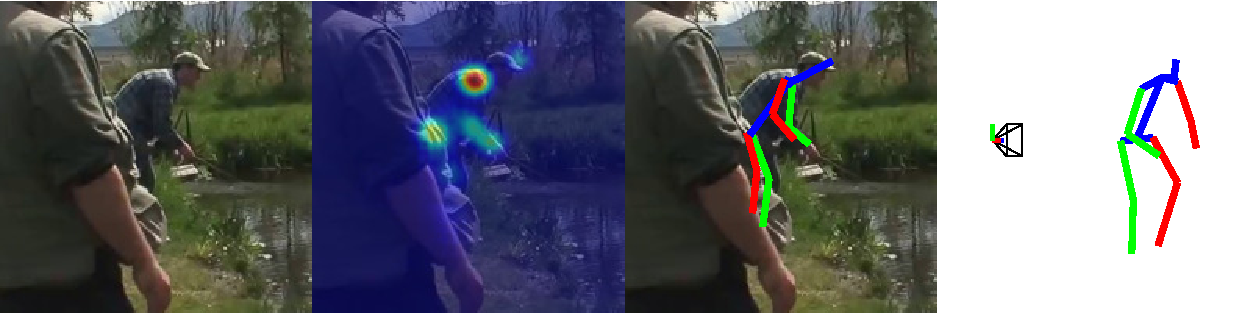
\includegraphics[width=0.48\linewidth]{figures/examples/mpii/mpii-016.pdf}
  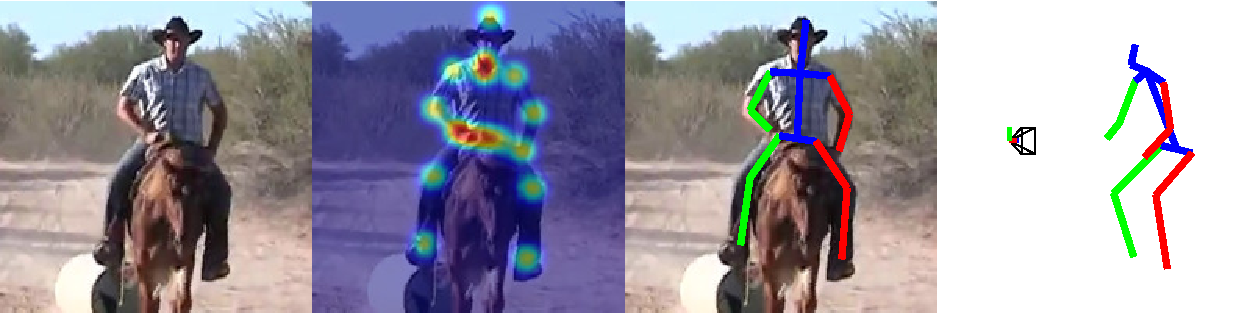
\includegraphics[width=0.48\linewidth]{figures/examples/mpii/mpii-022.pdf}
  %\includegraphics[width=0.48\linewidth]{figures/examples/mpii/mpii-035.pdf}
  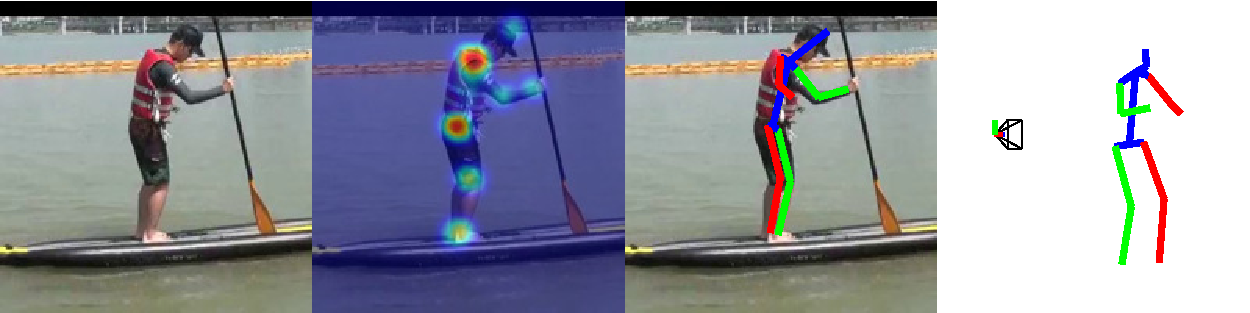
\includegraphics[width=0.48\linewidth]{figures/examples/mpii/mpii-043.pdf}
  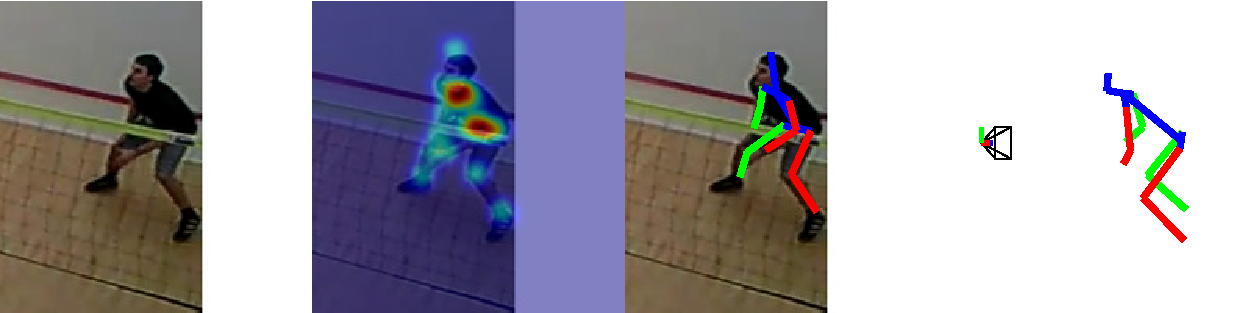
\includegraphics[width=0.48\linewidth]{figures/examples/mpii/mpii-044.pdf}
  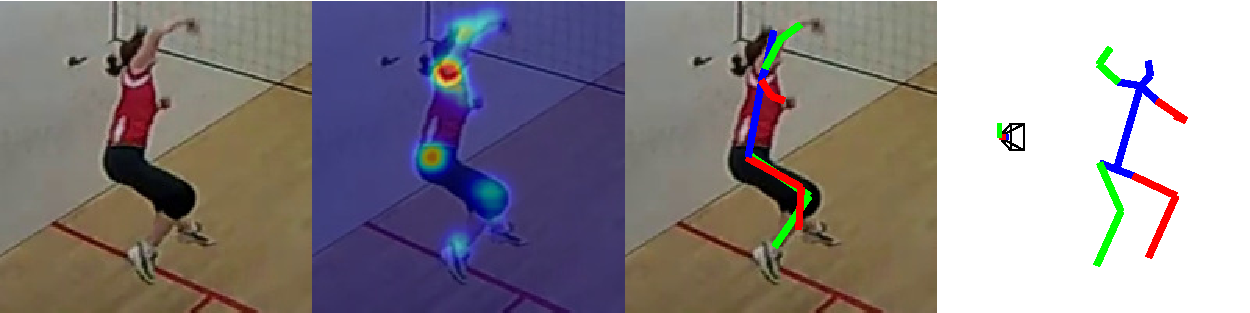
\includegraphics[width=0.48\linewidth]{figures/examples/mpii/mpii-052.pdf}
  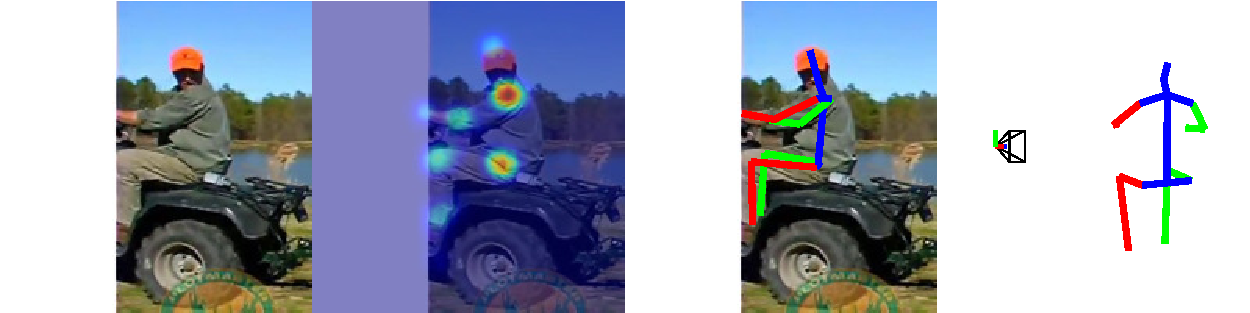
\includegraphics[width=0.48\linewidth]{figures/examples/mpii/mpii-053.pdf}
  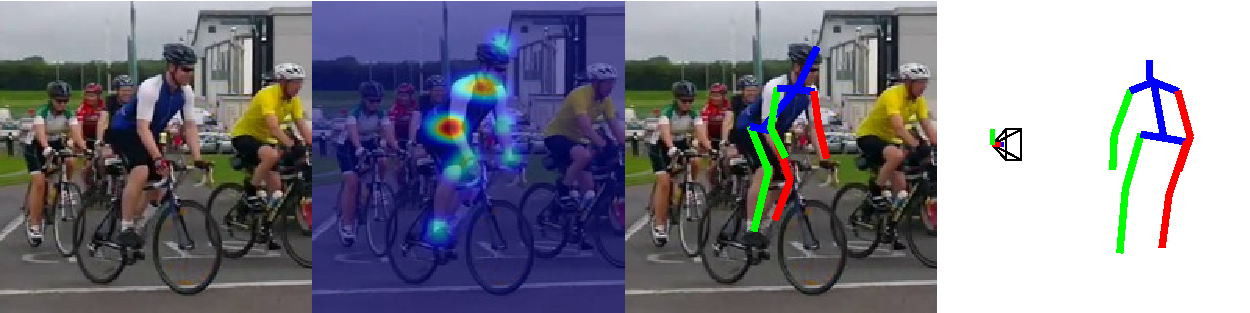
\includegraphics[width=0.48\linewidth]{figures/examples/mpii/mpii-057.pdf}
  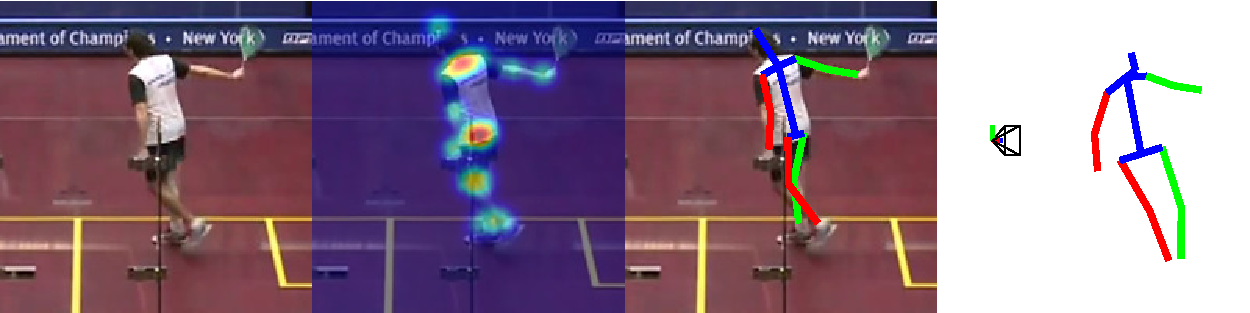
\includegraphics[width=0.48\linewidth]{figures/examples/mpii/mpii-060.pdf}
  % \includegraphics[width=0.48\linewidth]{figures/examples/mpii/mpii-090.pdf}
  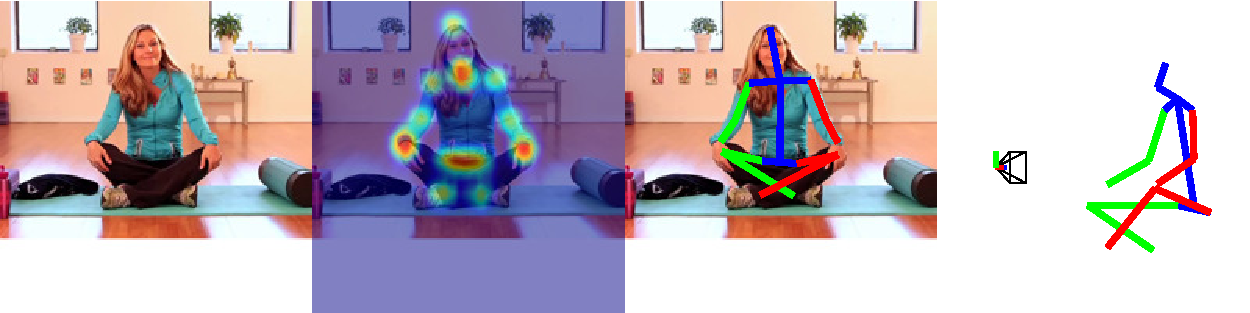
\includegraphics[width=0.48\linewidth]{figures/examples/mpii/mpii-124.pdf}
  %\includegraphics[width=0.48\linewidth]{figures/examples/mpii/mpii-140.pdf}
  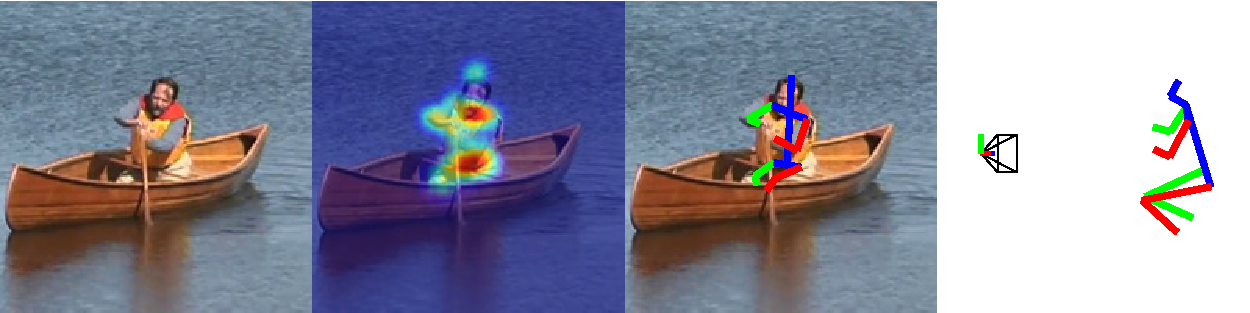
\includegraphics[width=0.48\linewidth]{figures/examples/mpii/mpii-150.pdf}
  %\includegraphics[width=0.48\linewidth]{figures/examples/mpii/mpii-188.pdf}
  \caption{关于MPII\cite{andriluka14cvpr}的成功案例。 在每个示例中,从左到右的图像对应于输入图像,热图(所有关节同时显示),估计的2D姿势,以及在新颖视图中可视化的估计3D姿势。 还显示了原始视点。}\label{fig:mpii-good}
\end{figure*}

最后,使用MPII Human Pose数据集\cite{andriluka14cvpr}定性地说明了我们提出的野外图像方法的适用性。 MPII是一个大型2D人体姿势数据集,包括从YouTube视频中提取的25K单个图像,其中包含超过40,000人和410个活动。 此数据集不包含3D姿势数据。
%No 3D pose data is available in the dataset. 
在该数据集上训练的原始沙漏模型\cite{newell2016stacked}被用作2D检测器并且与在Human3.6M上学习的非特定动作姿势字典组合以重建3D人体姿势。测试图像来自先前工作中定义的验证集 \cite{newell2016stacked}。

\refFig{fig:mpii-good}展示了MPII的成功案例。 请注意,输入数据由单个图像而不是序列组成。 当从另一个数据集学习姿势字典时,所提出的方法能够从单个图像产生视觉上合理的3D重建,用于各种各样的活动和视点。 \refFig{fig:mpii-improve}提供了一些在2D热图中具有较大不确定性的示例,如果关节仅由热图响应确定,则会导致不正确的2D姿势。 在通过所提出的方法对先前的3D姿势进行积分之后,获得了更好的姿势估计。\refFig{fig:mpii-bad}提供了几个失败的例子。 对这些结果的目视检查表明,失败主要是由于严重的遮挡,左右对称的模糊,重叠的人以及极其罕见的3D姿势,超出了学习姿势字典的代表能力。
%could hardly be represented by the pose dictionary.

\begin{figure*}
  \centering
  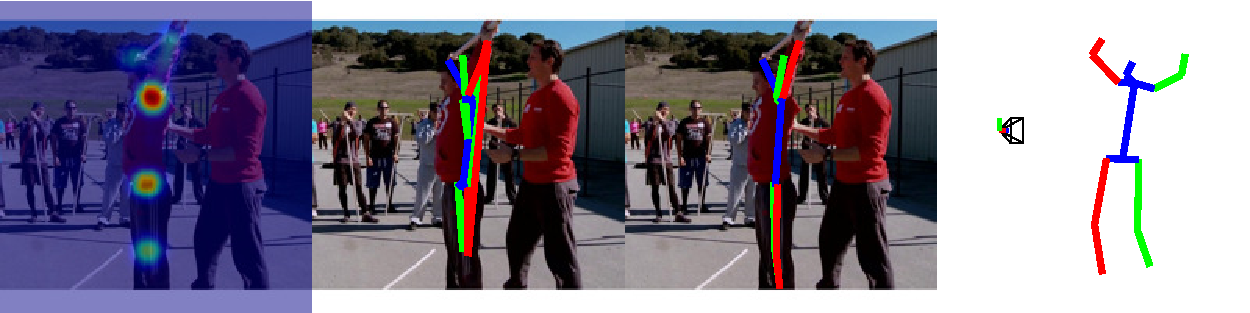
\includegraphics[width=0.48\linewidth]{figures/examples/mpii/pos-002.pdf}
  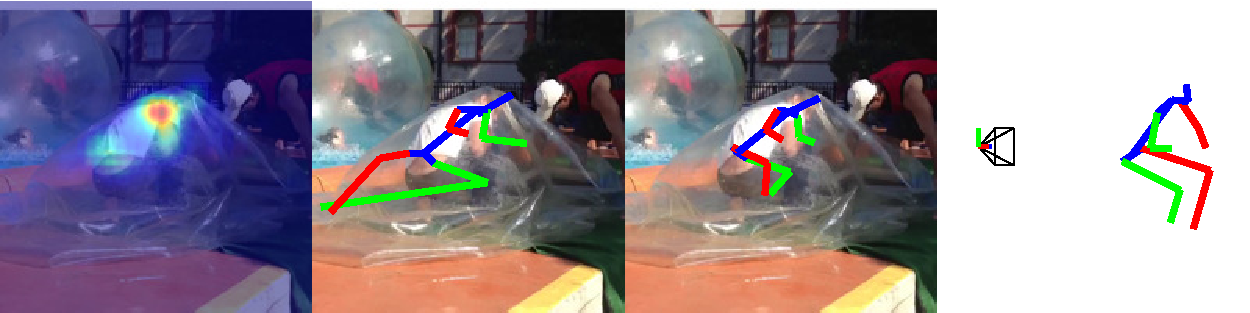
\includegraphics[width=0.48\linewidth]{figures/examples/mpii/pos-003.pdf}
  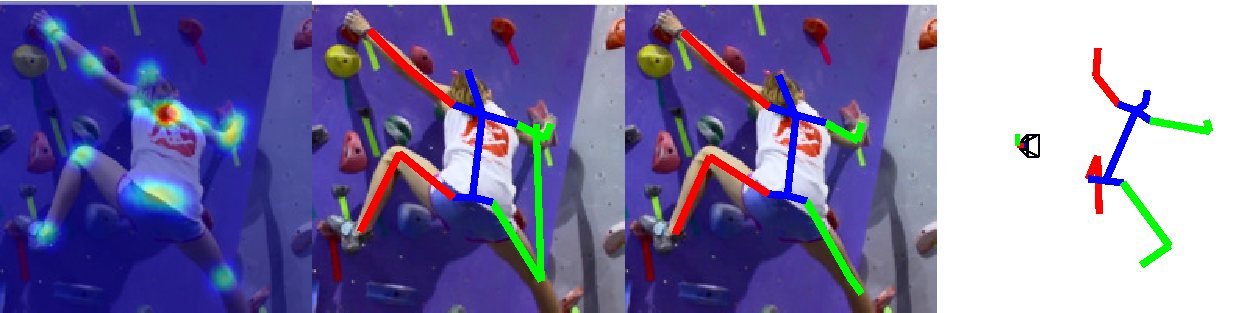
\includegraphics[width=0.48\linewidth]{figures/examples/mpii/pos-006.pdf}
  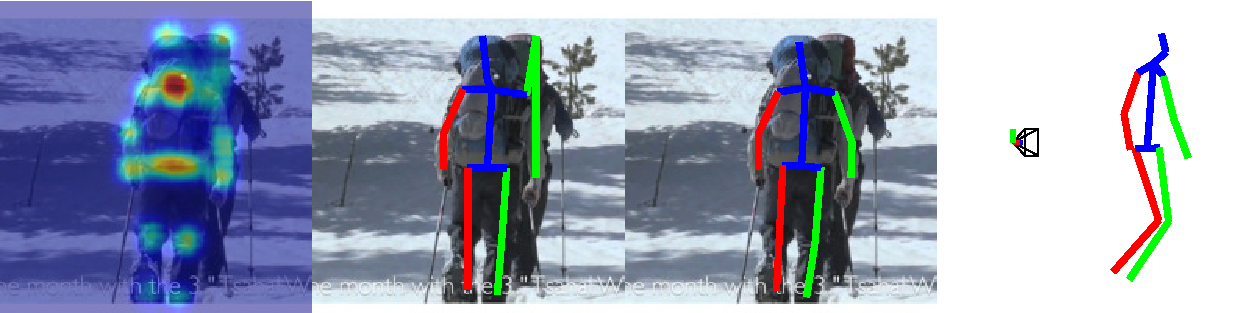
\includegraphics[width=0.48\linewidth]{figures/examples/mpii/pos-015.pdf}
  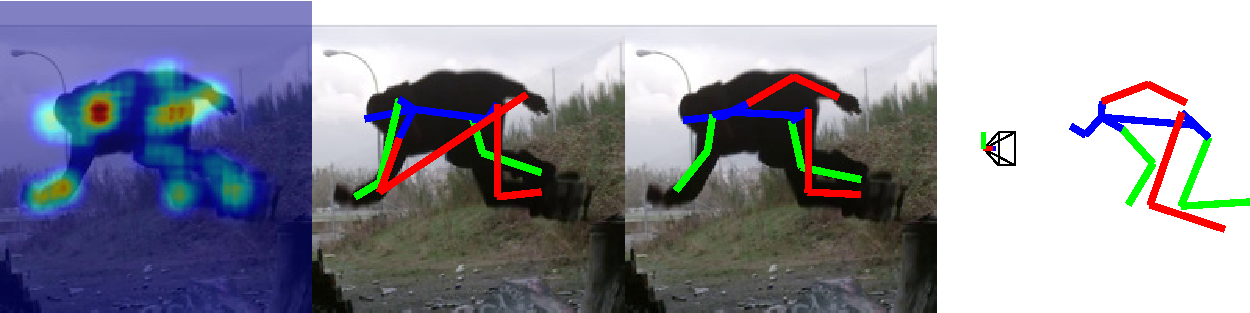
\includegraphics[width=0.48\linewidth]{figures/examples/mpii/pos-009.pdf}
  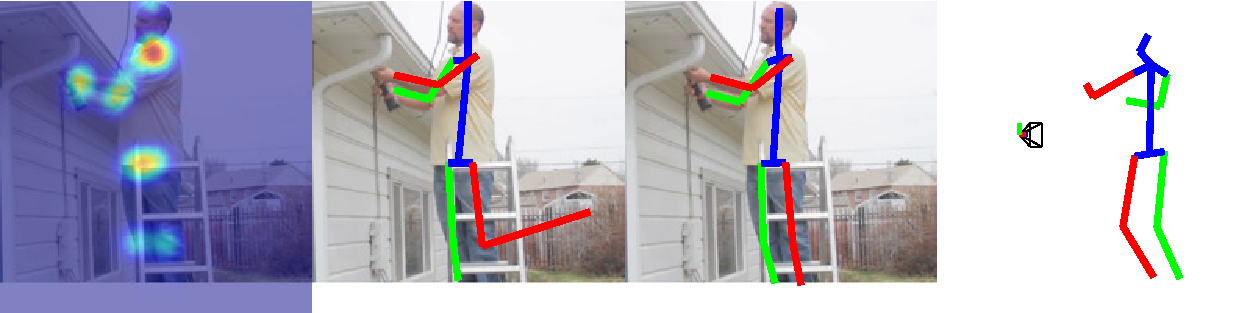
\includegraphics[width=0.48\linewidth]{figures/examples/mpii/pos-014.pdf}
  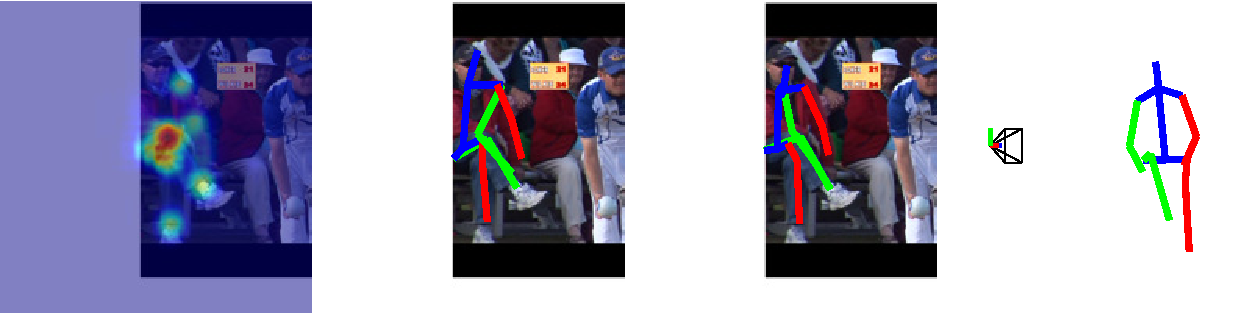
\includegraphics[width=0.48\linewidth]{figures/examples/mpii/pos-023.pdf}
  \includegraphics[width=0.48\linewidth]{figures/examples/mpii/pos-039.pdf}
  \caption{MPII\cite{andriluka14cvpr}的比较结果示例。 在每个示例中,从左到右的图像对应于热图(所有关节同时显示),通过根据热图分别贪婪地定位每个关节而发现的2D姿势,通过所提出的EM算法估计的2D姿势, 并且在新颖的视图中可视化估计的3D姿势。 还显示了原始视点。 请注意,在考虑3D姿势先验后,2D热图中的误差会得到纠正。}\label{fig:mpii-improve}
\end{figure*}


\begin{figure*}
  \centering
  % Requires \usepackage{graphicx}
  \includegraphics[width=0.48\linewidth]{figures/examples/mpii/bad-042.pdf}
  \includegraphics[width=0.48\linewidth]{figures/examples/mpii/bad-007.pdf}
  \includegraphics[width=0.48\linewidth]{figures/examples/mpii/bad-008.pdf}
  \includegraphics[width=0.48\linewidth]{figures/examples/mpii/bad-025.pdf}
  \caption{MPII\cite{andriluka14cvpr}上的失败示例。 在每个示例中,从左到右的图像对应于输入图像,热图(所有关节同时显示),估计的2D姿势,以及在新颖视图中可视化的估计3D姿势。 还显示了原始视点。 }\label{fig:mpii-bad}
\end{figure*}

\subsection{运行时间}

实验在台式机上进行,配备Intel i7 3.4G CPU,8GB RAM和GeForce GTX Titan X 6GB GPU。
基于CNN的热图生成(使用沙漏模型)和凸初始化的运行时间分别约为每帧0.3秒和0.6秒; 这两个步骤都可以轻松并行化。 对于300帧的序列,EM算法通常在20次迭代中收敛,CPU时间小于100s。我们的方法的运行时间取决于字典大小。 在准确性和效率之间进行权衡。 例如,对于字典大小为32,64,96和128
在S9的第一个“方向”序列上测试,平均重建误差(mm)分别为48.1,46.0,45.6和44.4,计算时间(秒)分别为91,197,317和488。